\documentclass[a4paper,10pt]{article}
\usepackage{My_math_package}

\title{MATH808K - Algebraic K-Theory} % password: 
\author{Haoran Li}
\date{2020 Spring}

\makeindex[columns=2, title=Index, intoc] % Create the index

\begin{document}\sloppy % Reduce overlong words

% Maketitle
\begin{titlepage}
\begin{center}
\vspace*{1cm}
\Huge
\textbf{MATH808Q - Abelian varieties} \\
\vspace{2cm}
% \begin{center}
% 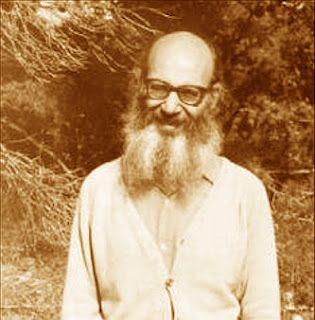
\includegraphics{Pictures/Grothendieck.jpg}
% \end{center}
\vspace{2cm}
\normalsize
Taught by \texttt{Ramachadran} \\
Notes taken by \texttt{Haoran Li} \\
2021 Fall \\
\vspace{2cm}
Department of Mathematics\\
University of Maryland\\
\end{center}
\end{titlepage}

% Contents
\tableofcontents
\newpage

\section{Introduction to Abelian varieties}
Motivating example: $V\cong\mathbb C^g$, $\Lambda\leq V$ is a lattice(discrete cocompact subgroup), $V\otimes_{\mathbb Z}\mathbb R=V$, $G=V/\Lambda$ is a compact complex abelian Lie group, a complex torus since $V/\Lambda\cong (S^1)^{2g}$

\begin{theorem}
Any compact connected(connected is necessary, otherwise finite groups would all be abelian) complex Lie group $X$ is abelian
\end{theorem}

\begin{proof}
$n=\dim_{\mathbb C}X$. Let $e\in U\subseteq\mathbb C^n$ be an open subset of $X$, $\phi_g:X\to X,x\mapsto gxg^{-1}$ induces $\phi:X\to\Aut(X)$, for a fixed $g\in X$,
\end{proof}

\begin{proof}
Consider $\phi:X\times X\to X,(x,y)\mapsto xyx^{-1}y^{-1}$, open neighborhood $V_g$ of $g$ and open neighborhood $W_g$ of $e$ such that $\phi(V_g,W_g)\subseteq U$ and $\phi(g,e)=e$. Since $X$ is compact, $X=\bigcup_{i=1}^rV_{g_i}$, let $W=\bigcap W_{g_i}$, then $\phi(X,W)\subseteq U$, is homomorphic, hence $\phi(X,W)=e$
\end{proof}

Every such group would be like $X=V/\Lambda$, $V=\Lie X=\tilde X$, and $\Lambda=\pi_1(X,e)=H_1(X,\mathbb Z)$. This is a complex tori, consider $X\xrightarrow nX$, let $X[n]\cong(\mathbb Z/n\mathbb Z)^{2g}$ denote the kernel which consists of $n$-torsion elements, this is an isogeny of degree $n^{2g}$

How to classify all such $X$, $\phi X=V/\Lambda\to X'=V'/\Lambda'\Leftrightarrow \tilde\phi:V\to V'$ and $\tilde \phi(V)\subseteq V'$, need to consider something like $\GL_g(\mathbb C)/\GL_g(\mathbb C)\cap\GL_{2g}(\mathbb Z)$

Tate module $T_pA\cong(\mathbb Z_p)^{2g}$

\begin{definition}
$F$ is a perfect field with $F=\overline F$, an abelian variety $A$ is a group variety that is proper(irreducible, reduced, connected)
\end{definition}

\begin{lemma}[Rigidity]\label{Rigidity lemma}
Suppose $X$ is proper, $f:X\times Y\to Z$ is a morphism such that $f(X\times y_0)=z_0\in Z$, then $f(X\times y)$ is a point in $Z$ for any $y\in Y$
\end{lemma}

\begin{proof}
Just need to show that there exists a unique map $g:Y\to Z$ such that $f=gp_2$, and it suffices to show that $f=gp_2$ on a nonempty open set of $X\times Y$. Since $f(X\times y_0)=z_0$, there exists nonempty closed $W\subseteq Z$ such that $f^{-1}(W)$ is disjoint from $X\times y_0$, and since $X$ is proper, $X\times Y\to Y$ is closed, so $Y'=p_2(f^{-1}(W))$ is closed, and $V=Y-Y'$ is a nonempty open set in $Y$ containing $y_0$, for any $y\in V$, $f(X\times y)\subseteq U=Z-W$ open, but $X\times y\cong X$ is proper, hence $f(X\times y)$ is a point, denote as $g(y)$, then $f=gp_2$ on $X\times V\subseteq X\times Y$
\end{proof}

\begin{remark}
Note that the lemma is false if $X$ is not proper, for example $\mathbb A^1\times\mathbb A^1\to\mathbb A^1,(x,y)\mapsto xy$
\end{remark}

\begin{theorem}[Chevalley]
There is an exact sequence(in general non split)
\[1\to H\to G\to A\to 1\]
$A$ is an abelian variety, $H$ is affine
\end{theorem}

\begin{theorem}
Any abelian variety $A$ is commutative(hence the term "abelian")
\end{theorem}

\begin{proof}
Consider $f:A\times A\to A,(x,y)\mapsto xyx^{-1}y^{-1}$, then $f(A,e)=e$, by Lemma \ref{Rigidity lemma}, $f(A,y)=f(e,y)=e$, thus $A$ is commutative
\end{proof}

\begin{corollary}
$A$ is an abelian variety, $G$ is a group variety, $f:A\to G$ is a morphism with $f(e_A)=e_G$, then $f$ is a group homomorphism
\end{corollary}

\begin{proof}
Consider $\phi:A\times A\to G$, $(x,y)\mapsto f(x)f(y)f(xy)^{-1}$, then $\phi(A,e_A)=e_G$, by Lemma \ref{Rigidity lemma}, $\phi(x,y)=\phi(e_A,y)=e_G$, hence $f$ is a homomorphism
\end{proof}

\begin{corollary}
$A$ is an abelian variety, $X,Y$ are proper varieties pointed at $x_0,y_0$, then there is a bijection
\[\Hom(X,A)\times \Hom(Y,A)\to\Hom(X\times Y,A),\quad (f,g)\mapsto f+g\]
\end{corollary}

\begin{proof}
This is injective since $f(x)=h(x,y_0)$, $g(y)=h(x_0,y)$. This is also surjective by define $f,g$ the same way and consider $k(x,y)=h(x,y)-f(x)-g(y)$
\end{proof}

\begin{definition}
$S$-group scheme. $G$ is commutative if $m$ is a symmetric
\end{definition}

\begin{exercise}
$G\to S$ is separable iff $e:S\to G$ is a closed immersion
\end{exercise}

\begin{definition}
$f:G\to H$ is a $S$-group scheme homomorphism if it is compatible with $m,i,e$, $\ker f$ as the pullback of $G\xrightarrow{f} H$ and $S\xrightarrow{e_H}H$ is again a $S$-group scheme, and $(\ker f)(T)=\ker(f_T)$
\end{definition}

An abelian variety doesn't in general have a Hopf algebra structure, but due to Mumford, we can use Heisenberg group, or Mumford Tate group to help us study and understand

A group scheme can be reduced, for example $\Spec\mathbb F_p[t]/(t^p)$. However we have

\begin{theorem}[Oort]
$char k=0$, then any group scheme over $k$ is reduced
\end{theorem}

$X$ is a compact complex Lie group, $g=\dim X$, $H^0(X,\Omega^1)\cong\mathbb C^g$, $H_1(X,\mathbb Z)\to H^0(X,\Omega^1)^*$ with the image being a lattice $\Lambda$, $X\xrightarrow{\cong} H^0(X,\Omega^1)^*/\Lambda=V/\Lambda$, $V=\Lie X\cong\tilde X$ by sending $p\in X$\ to $\int_0^p$

If $\phi:X_1\to X_2$ is a holomorphic, $\phi(0)$, $\phi(e_{X_1})=e_{X_2}$, then $\phi$ is a homomorphism

\begin{proof}
\begin{tikzcd}
{H_1(X_1,\mathbb Z)} \arrow[d] \arrow[r] & {H^0(X_1,\Omega^1)^*} \arrow[d] \arrow[r] & V_1/\Lambda_1 \arrow[d] & X_1 \arrow[l] \arrow[d] \\
{H_1(X_2,\mathbb Z)} \arrow[r]           & {H^0(X_2,\Omega^1)^*} \arrow[r]           & V_2/\Lambda_2           & X_2 \arrow[l]          
\end{tikzcd}
\end{proof}

This means any holomorphic map $\phi:X_1\to X_2$ is homomorphism + translation
\begin{center}
\begin{tikzcd}
                                                                                         & {\Hom_{\mathbb C}(V_1,V_2)}                   \\
{\Hom(X_1,X_2)} \arrow[ru, "\varphi_{\mathbb C}", hook] \arrow[r, hook] \arrow[rd, hook] & {\Hom_{\mathbb Z}(\Lambda_1,\Lambda_2)}       \\
                                                                                         & {\Hom(H_1(X,\mathbb Z_p),H_1(X,\mathbb Z_p))}
\end{tikzcd}
\end{center}
$\phi\in\Hom(X_1,X_2)$ determines $\tilde\phi:V_1\to V_2$, and $\phi(\Lambda_1)\subseteq\Lambda_2$, thus makes $\varphi_{\mathbb Z}$ injective, and $\Hom_{\mathbb Z}(\Lambda_1,\Lambda_2)$ is of rank $(2\dim X_1)(2\dim X_2)$, hence we know $\Hom(X_1,X_2)$ is finite, in fact, $\End(X)$ will be a free $\mathbb Z$-algebra of rank $4\dim X^2$. We also have $\im\varphi\subseteq X_2$ is a subtorus, $\ker\varphi$ is a subtorus

\begin{definition}
$\phi:X_1\to X_2$ is an isogeny if $\phi$ is surjective and $\ker\phi$ is finite, define $\deg\phi=|\ker\phi|<\infty$
\end{definition}

Composition of isogeny is again an isogeny, deg multiply

$X_1\sim X_2$ isogeny is an equivalence relation. Suppose $\phi:X_1\to X_2$ is an isogeny of deg $n$, then there exists a unique isogeny $\phi^*:X_2\to X_1$

Consider

\begin{center}
\begin{tikzcd}
X_1 \arrow[rd, "n"] \arrow[r, "\phi"] & X_2 \arrow[d, "\phi^*"] \\
                                      & X_1                    
\end{tikzcd}
\end{center}

since homo, we have
\begin{center}
\begin{tikzcd}
X_1 \arrow[r, "\phi"] \arrow[r] \arrow[d, "n"] & X_2 \arrow[d, "n"] \\
X_1 \arrow[r, "\phi"]                          & X_2               
\end{tikzcd}
\end{center}

$(\phi\phi^*-n)\phi=0$ and $\phi$ is surjective

By Chow's theorem, any analytic variety $V$ in $\mathbb CP^n$ is an algebraic variety, and thus a group variety(The graph $m:V\times V\to V$ being $V\times V\times V$ being an analytic variety that can be embedded in $\mathbb CP^N$), actually an abelian variety(being proper)

Let $V$ be a dimension $g$ complex vector space, $H:V\times V\to\mathbb C$ is a Hermitian form, $H=S+iE$, $S=Re H$, $E=Im H$, then

$X=V/\Lambda$ is an abelian variety, $E|_{\Lambda\times\Lambda}:\Lambda\times\Lambda\to\mathbb Z$ is a bilinear $\mathbb Z$ valued map, then we say that $E$ is a Riemann form

\begin{example}
$X=\mathbb C/\Lambda$, where $\Lambda=\mathbb Z\lambda_1+\mathbb Z\lambda_2$, define $E$ such that $z\wedge w=E(z,w)\lambda_1\wedge\lambda_2$, 
\end{example}

\begin{example}
Suppose $K/\mathbb Q$ is a CM field(totally imaginary field), $K^+/\mathbb Q$ is the totally real field. $\Phi:K\otimes_{\mathbb Q}\mathbb R\to\mathbb C^g$ is an embedding. Nonzero ideal $I\subseteq \mathcal O_K$ are both lattices, say $\Phi(\mathcal O_K)$ is $\Lambda$, $X=\mathbb C^g/\Lambda$ is called a CM abelian variety, $\mathcal O_K\hookrightarrow\End(X)$ are multiplications. It is a fact that $K=K^+(\xi)$ with $-\xi^2\in K^+$ totally positive and $Im(\phi_j(\xi))>0$. For $z,w\in\mathbb C^g$, define $E(z,w)=\sum_j\phi(g_j)(\bar z_jw_j-z_j\bar w_j)$, for $\alpha,\beta\in\mathcal O_K$, $E(\Phi(\alpha),\Phi(\beta))=Tr_{K/\mathbb Q}(\xi\tilde\alpha\beta)$, here $K\to K, x\mapsto\tilde x$ is the unique automorphism fixing $K^+$
\end{example}

\begin{center}
\begin{tikzcd}
V\times\mathbb C\cong\pi^* L \arrow[d] \arrow[r] & L \arrow[d] \\
V \arrow[r, "\pi"]                               & X          
\end{tikzcd}
\end{center}

$\pi^*L$ is holomorphically trivial because the exponential sequence $0\to 2\pi i\mathbb Z\to\mathcal O_V\to\mathcal O_V^\times\to0$

Consider the group action of $\Lambda$ on $V$, and corresponding action $\Lambda$ on $V\times\mathbb C$ defined as $(z,t)\cdot\lambda=(z+\lambda,e_\lambda(z)t)$, here $e_\lambda\in\mathbb O_V^\times$ satisfying the cocycle condition $e_{\lambda_1+\lambda_2}(z)=e_{\lambda_2(z+\lambda_1)}e_{\lambda_1}(z)$, note that this is commutative


Let $F$ be a number field, with $r_1$ real embeddings and $2r_2$ complex embeddings, $r_1+2r_2=[F:\mathbb Q]$, let $w_F$ be the number of roots of unity, $h_F=|\Cl(\mathcal O_F)|$ be the class number of $F$, $r_F$ is the regulator of $F$ which is the covolume of the lattice $\mathcal O_F^\times/\text{torsion}\hookrightarrow\mathbb R^{r_1+r_2-1}$. We can the define the zeta function
\[
\zeta_F(s)=\sum_{0\neq\mathfrak I\leq\mathcal O_F}\frac{1}{|\mathfrak I|^s}=\prod_{\mathfrak p\text{ prime}}\frac{1}{1-|\mathfrak p|^s},\quad \operatorname{Re}s>1
\]

\begin{theorem}
$\zeta_F(s)$ admits analytic continuation to all of $\mathbb C$ with a simple pole at $s=1$, so $(s-1)\zeta_F(s)$ is analytic, and it satisfies the functional relation $\zeta_F(s)=2^s\pi^{s-1}\sin(\frac{\pi s}{2})\Gamma(1-s)\zeta_F(1-s)$. Denote
\[
\zeta_F^*(1)=\Res_{s=1}\zeta_F(s)=\pm\frac{2^{r_1}(2\pi)^{r_2}h_Fr_F}{w_F\sqrt{|d_F|}}
\]
\end{theorem}

$F=\mathbb Q(\sqrt{-d})$, $d>0$, $r_F=1$, $\zeta_F^*(1)=2\pi h_F$

$F=\mathbb Q(\sqrt{d})$, $d>0$, $\mathcal O_F^\times=\pm\varepsilon_F^{\mathbb Z}$, $\varepsilon_F$ is the fundamental unit, $\zeta_F^*(1)=\frac{h_F\log(\varepsilon_F)}{\sqrt{|d_F|}}$. $h_F$ is a global invariant

$C/\mathbb F_q$ is a smooth projective curve, geometrically connected
\[
\zeta(C,s)=\prod_{x\in C\text{ closed points}}\frac{1}{1-N(x)^{-s}}=\prod_x\frac{1}{1-(q^{-s})^{\deg x}}
\]
here $N(x)=[k(x):k]=q^{\deg s}$. Write $Z(C,t)=\prod_x\frac{1}{1-t^{\deg x}}$, then $\zeta(C,s)=Z(C,q^{-s})$

$Z(C,t)=\frac{P_1(t)}{(1-t)(1-qt)}$, $P_1(t)\in\mathbb Z[t]$ of degree $2g$, $g$ is the genus of $C$

\begin{theorem}[Weil, Emil Artin, Hasse]
$s=1$, $t=1/q$, $(1-qt)Z(C,t)|_{t=1/q}=\frac{P_1(1/q)}{1-1/q}=\frac{h_C}{q-1}q^{1-g}$, here $h_C$ is the class number which is $\#J(C)(\mathbb F_q)$($J$ is the Jacobian), $q-1$ is like $w_C$, $q^{g-1}$ is like $\sqrt{|d_C|}$
\begin{center}
\begin{tikzcd}
C \arrow[d] \arrow[r]      & \Spec\mathcal O_F \arrow[d] \\
\Spec\mathbb F_p \arrow[r] & \Spec\mathbb Z             
\end{tikzcd}
\end{center}
\end{theorem}

We generalize in dimension 2 $\mathcal E\subseteq\mathbb P^2_{\mathbb Z}$
\begin{center}
\begin{tikzcd}
E \arrow[d] \arrow[r]    & \mathcal E \arrow[d] \\
\Spec\mathbb Q \arrow[r] & \Spec\mathbb Z      
\end{tikzcd}
\end{center}

In Tate's thesis, he dealt with $F$ number field, $\mathbb F_q(C)$

$\mathbb Z=\prod_p\mathbb Z_p$, $A_{\mathbb Q}^f=\widehat{\mathbb Z}\otimes_{\mathbb Z}\mathbb Q\subseteq\prod\mathbb Q_p$, $A_{\mathbb Q}^f=(\widehat{\mathbb Z}\otimes_{\mathbb Z}\mathbb Q)\times\mathbb R\subseteq(\prod\mathbb Q_p)\times\mathbb R$, $\mathbb A_F=\mathbb A_Q\otimes_{\mathbb Q}F$ for a number field $F$, $\mathbb G_m(\mathbb A_F)=\mathbb I_F$, we have diagonal maps $F\xrightarrow{\Delta}\mathbb A_F$, $F^\times\xrightarrow{\Delta}\mathbb I_F$, $\left|\frac{\mathbb G_m(\mathbb A_F)^1}{\mathbb G_m(F)}\right|$ is finite and arithmetically interesting, here $\mathbb I_F^1$ is the kernel of $\mathbb I_F\to\mathbb R^\times$, $x\mapsto N(x)$

Andr\'e Weil considered $\left|\frac{G(\mathbb A_F)^1}{G(F)}\right|$ for $G/F$ is an algebraic group(e.g. $G=\SL_n,\SO_n$), and reintepreted the result of Siegel on quadratic forms

$E/\mathbb Q$ is an elliptic curve, since $E(\mathbb Q_p)=E(\mathbb Z_p)$, $\mathbb P^n(\mathbb Q)=\mathbb P^n(\mathbb Z)$, $\frac{E(\mathbb A_{\mathbb Q})}{E(\mathbb Q)}=\frac{E(\widehat{\mathbb Z})\times E(\mathbb R)}{E(\mathbb Z)}$ is not Hausdorff if $\rank E\mathbb (Q)>0$

BSD conjecture: $E/F$ is an elliptic curve(Abelian variety), $L(E,s)=\prod L_p(E,s)$, $\operatorname{Re}s>\frac{3}{2}$ has a analytic continuation to all of $\mathbb C$, $\ord_{s=0}L(F,s)=\rank\mathcal O_F^\times$

Weak: $\ord_{s=1}L(E,s)=\rank E(F)$

Strong: $L^\times(E,s)$

\begin{thebibliography}{}



\end{thebibliography}

\printindex
\newpage

\end{document}